\color{black}
\subsection{Specifica componenti View::Dialog}
\label{specificaDialog}
\begin{figure}[!h]

			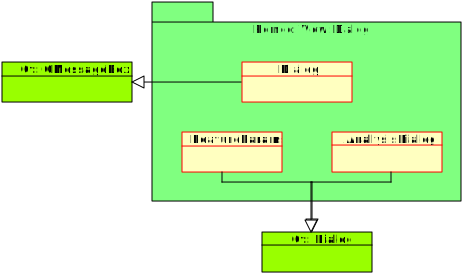
\includegraphics[width=0.7\linewidth]{../Specifica_Tecnica/Content/Immagini/Romeo__View__Dialog.png}
			\caption{Componente Romeo::View::Dialog}
			\label{comp_romeo::view::dialog}
\end{figure}
Componente che contiene tutte le classi che rappresentano le finestre di dialogo con cui l'utente potrà interagire
\pagebreak
%%%%%%%%%%%%%%%%%%%5
% 	DIALOG
%%%%%%%%%%%%%%%%%
\subsubsection{Dialog (class)}
\label{spedialog}
\begin{figure}[!h]
\centering
			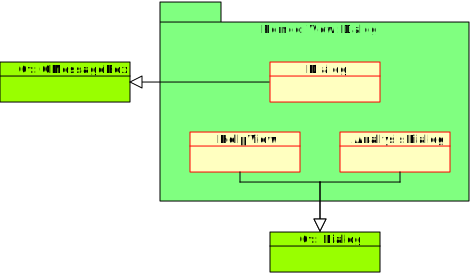
\includegraphics[width=1.1\linewidth]{./Content/Immagini/view/Dialog.png}
			\caption{Classe Dialog: attributi e metodi}
			\label{cl_dia}
\end{figure}
\paragraph{Descrizione \\}
Classe che rappresenta le varie finestre di dialogo che mandano all'utente un messaggio, e che attende la pressione di un pulsante da parte dell'utente per proseguire. Possono essere messaggi che se accettati, interrompono la regolare operazione che era in esecuzione prima dell'apertura del messaggio di dialogo.
\paragraph{Utilizzo\\}
La classe viene utilizzata per dare messaggi all'utente.
\paragraph{Classi ereditate\\}
\begin{itemize}
\item Qt::QMessageBox.
\end{itemize}
%%%%%%%%%  METODI
\paragraph{\textcolor{black}{Metodi\\}}
%costruttore
\color{blue}\verb!- Dialog(title:QString&, text:QString&, info:QString&, detail:QString&, parent:QWidget*=0)!
\begin{quote}
\color{black}Costruttore privato per la classe Dialog. Viene invocato dai metodi statici che mette a disposizione la classe in esame. \\
\textbf{Argomenti}
\begin{itemize}
\item title: QString\& \\ title viene settato come titolo della finestra di dialogo;
\item text: QString\& \\ text viene utilizzato per impostare il testo della finestra di dialogo;
\item info: QString\& \\ info viene utilizzato per impostare le informazioni della finestra di dialogo;
\item detail: QString\& \\ detail viene utilizzato per impostare i dettagli che la finestra di dialogo fornisce all'utente;
\item parent: QWidget*=0  \\ Puntatore al QWidget padre di Dialog.
\end{itemize}
\end{quote}
%dialogInfo
\color{blue}\verb! + static dialogInfo(title:QString&, text:QString&, info:QString&,! \\ \verb! detail:QString&, parent:QWidget * = 0): int!
\color{black}
\begin{quote}
Metodo statico che invoca la creazione di una finestra di dialogo che da un messaggio informativo. Ritorna il numero del pulsante che l'utente ha premuto. \\
\textbf{Note:}
\begin{itemize}
\item Questo metodo deve essere marcato statico.
\item Gli argomenti del metodo, vengono passati al costruttore della classe \emph{Dialog}.
\end{itemize}
\end{quote}
%dialogCritical
\color{blue}\verb! + static dialogCritical(title:QString&, text:QString&, info:QString&,! \\ \verb! detail:QString&, parent:QWidget * = 0): int!
\color{black}
\begin{quote}
Metodo statico che invoca la creazione di una finestra di dialogo che da un messaggio di criticità. Ritorna il numero del pulsante che l'utente ha premuto. \\
\textbf{Note:}
\begin{itemize}
\item Questo metodo deve essere marcato statico.
\item Gli argomenti del metodo, vengono passati al costruttore della classe \emph{Dialog}.
\end{itemize}
\end{quote}
%dialogQuestion
\color{blue}\verb! + static dialogQuestion(title:QString&, text:QString&, info:QString&,! \\ \verb! detail:QString&, parent:QWidget * = 0): int!
\color{black}
\begin{quote}
Metodo statico che invoca la creazione di una finestra di dialogo che richiede una risposta da parte dell'utente. Ritorna il numero del pulsante che l'utente ha premuto. \\
\textbf{Note:}
\begin{itemize}
\item Questo metodo deve essere marcato statico.
\item Gli argomenti del metodo, vengono passati al costruttore della classe \emph{Dialog}.
\end{itemize}
\end{quote}
%DialogWarning
\color{blue}\verb! + static dialogCritical(title:QString&, text:QString&, info:QString&,! \\ \verb! detail:QString&, parent:QWidget * = 0): int!
\color{black}
\begin{quote}
Metodo statico che invoca la creazione di una finestra di dialogo che da un messaggio di warning. Ritorna il numero del pulsante che l'utente ha premuto. \\
\textbf{Note:}
\begin{itemize}
\item Questo metodo deve essere marcato statico.
\item Gli argomenti del metodo, vengono passati al costruttore della classe \emph{Dialog}.
\end{itemize}
\end{quote}
\pagebreak
%%%%%%%%%%%%%%%%%%
% 	featureParams
%%%%%%%%%%%%%%%%%%%%
\subsubsection{FeatureParams (class)}
\label{speFeaPar}
\begin{figure}[!h]
\centering
			\includegraphics[width=0.8\linewidth] {./Content/Immagini/view/FeatureParams.png}
			\caption{Classe FeatureParams: attributi e metodi}
			\label{cl_fea}
\end{figure}
\paragraph{Descrizione \\}
Classe che rappresenta la finestra di dialogo che permette all'utente di impostare i valori dei parametri per una determinata Feature\g{}.
\paragraph{Utilizzo\\}
La classe viene utilizzata dalla finestra \emph{NewProtocolView} alla pressione del pulsante che permette l'inserimento di una nuova Feature\g{} nel \protocol in creazione. Dà la possibilità di impostare i valori dei parametri che richiede la Feature\g{}, dando comunque un valore di default per ogni parametro.
\paragraph{Classi ereditate\\}
\begin{itemize}
\item Qt::QDialog.
\end{itemize}

%%%%%%%%%%% ATTRIBUTI
\paragraph{\textcolor{black}{Attributi\\}}
%FEATURES
\color{teal}\verb!-features: QVector<AFeature*>!
\color{black}
\begin{quote}
Contiene la lista di tutte le Feature\g{} rese disponibili da \project.
\end{quote}
%params
\color{teal}\verb! - params:QStringList*!
\color{black} 
\begin{quote}
Lista contentente tutti i parametri richiesti dalla Feature\g{} che si vuole aggiungere.
\end{quote}
%type
\color{teal}\verb! - type:QString!
\color{black} 
\begin{quote}
Stringa che contiene il tipo della Feature\g{} che si sta creando.
\end{quote}
%feature
\color{teal}\verb! - feature: AFeature*!
\color{black} 
\begin{quote}Puntatore polimorfo alla Feature\g{} selezionata.
\end{quote}
%FeaturesComboBox
\color{teal}\verb! - featuresComboBox: ComboBox*!
\color{black} 
\begin{quote}Visualizza le Feature\g{} contenute nel campo dati \emph{features}.
\end{quote}
%firstWSize
\color{teal}\verb! - firstWSize: QLineEdit*!
\color{black} 
\begin{quote}Linea di testo per impostare la dimensione della finestra per la Feature\g{} di primo ordine.
\end{quote}
%secondWSize
\color{teal}\verb! - secondWSize: QLineEdit*!
\color{black} 
\begin{quote}Linea di testo per impostare la dimensione della finestra per la Feature\g{} di secondo ordine.
\end{quote}
%secondGlcm
\color{teal}\verb! - secondGlcm: QLineEdit*!
\color{black} 
\begin{quote}Linea di testo per impostare il valore della GLCM\g{}.
\end{quote}
%dynamicWSize
\color{teal}\verb! - dynamicWSize: QLineEdit*!
\color{black} 
\begin{quote}Linea di testo per impostare la dimensione della finestra per la Feature\g{} di tipo dinamico.
\end{quote}
%dynamicInitialFrame
\color{teal}\verb! - dynamicInitialFrame: QLineEdit*!
\color{black} 
\begin{quote}Linea di testo per impostare il frame iniziale per la Feature\g{} dinamica.
\end{quote}
%dynamicInitialFrame
\color{teal}\verb! - dynamicInitialFrame: QLineEdit*!
\color{black} 
\begin{quote}Linea di testo per impostare il frame finale per la Feature\g{} dinamica.
\end{quote}
%%%%%%%%%  METODI
\paragraph{\textcolor{black}{Metodi\\}}
%costruttore
\color{blue}\verb!- FeatureParams(featureP: QVector<AFeature*>&, parent:QWidget*=0)!
\begin{quote}
\color{black}Costruttore per la classe. \\
\textbf{Argomenti}
\begin{itemize}
\item featureP: QVector<AFeature*>\& \\ Vector di puntatori ad oggetti di tipo \emph{AFeature}. Utilizzato per inizializzare il campo dati \emph{features};
\item parent: QWidget*=0  \\ Puntatore al QWidget padre di FeatureParams.
\end{itemize}
\end{quote}
\color{blue}\verb! -setupLayout(): void !
\begin{quote}
\color{black} Metodo che ha il compito di impostare il layout del widget.
\end{quote} 
%LOADCSS
\color{blue}\verb! -loadCss(): void !
\begin{quote}
\color{black} Metodo che ha il compito di caricare il file contentente il css per il widget.
\end{quote} 
%setupObjectName
\color{blue}\verb! -setupObjectName():void!
\begin{quote}
\color{black} Metodo che ha il compito di impostare il nome di ogni oggetto, contenuto nel widget.
\end{quote} 
%setupToolTip
\color{blue}\verb! -setupToolTip():void!
\begin{quote}
\color{black} Metodo che ha il compito di impostare per ogni oggetto i ToolTip necessari per mostrare all'utente, che sta utilizzando \project{}, i suggerimenti e  spiegare a cosa serve quell'oggetto su cui si è posizionato con il cursore.
\end{quote} 
%addConnect
\color{blue}\verb! -addConnect(): void!
\color{black} 
\begin{quote}
Metodo che ha il compito di fissare tutte le istruzioni \emph{connect} degli oggetti che emetteranno un signal\g{} verso il rispettivo controller.
\end{quote} 
%setupView
\color{blue}\verb! -setupView(): void !
\begin{quote}
\color{black} Metodo che ha il compito di impostare il layout del widget.
\end{quote} 
%createTop
\color{blue}\verb! -createTop():void!
\begin{quote}
\color{black} Metodo che ha il compito di creare la parte in alto della finestra di dialogo contenente i campi per l'inserimento dei valori dei parametri per la Feature\g{} selezionata.
\end{quote} 
%createLayout
\color{blue}\verb! -createLayout():void!
\begin{quote}
\color{black} Metodo che ha il compito di creare il layout per la finestra di dialogo.
\end{quote} 
%createButtom
\color{blue}\verb! -createButtom():void!
\color{black}
\begin{quote}
 Metodo che ha il compito di costruire la parte in basso del widget contenente il pulsante per il salvataggio dei valori inseriti oppure per poter reimpostare la form.
\end{quote}
%createFeatureBox
\color{blue}\verb! -createFeatureBox():void!
\color{black}
\begin{quote}
 Metodo che ha il compito di costruire il box contenente i campi per l'inserimento delle informazioni necessarie.
\end{quote}
%createFirstBox
\color{blue}\verb! -createFirstBox():void!
\color{black}
\begin{quote}
 Metodo che ha il compito di costruire il box contenente i campi per l'inserimento delle informazioni necessarie, relative alle Feature\g{} di primo ordine.
\end{quote}
%createSecondBox
\color{blue}\verb! -createFirstBox():void!
\color{black}
\begin{quote}
 Metodo che ha il compito di costruire il box contenente i campi per l'inserimento delle informazioni necessarie, relative alle Feature\g{} di secondo ordine.
\end{quote}
%createDynamicBox
\color{blue}\verb! -createFirstBox():void!
\color{black}
\begin{quote}
 Metodo che ha il compito di costruire il box contenente i campi per l'inserimento delle informazioni necessarie, relative alle Feature\g{} dinamiche.
\end{quote}

%visibleBox
\color{blue}\verb! + visibleBox(type:QString&): void!
\color{black}
\begin{quote} Metodo che imposta la finestra di dialogo mostrando i campi corretti per l'inserimento dei valori dei parametri in base al valore della stringa passata come parametro al metodo.\\
\textbf{Argomenti}
\begin{itemize}
\item type: QString\& \\ rappresenta il tipo di Feature\g{} ovvero se di primo, secondo ordine o dinamica.
\end{itemize}
\end{quote}

%resetBox
\color{blue}\verb! + resetBox(): void!
\begin{quote}
\color{black} Metodo che reimposta la finestra di dialogo, mostrando solamente il menu di selezione con le Feature{} disponibili.
\end{quote}
%visibleBox
\color{blue}\verb! + visibleBox(type:QString&): void!
\color{black}
\begin{quote} Metodo che imposta la finestra di dialogo mostrando i campi corretti per l'inserimento dei valori dei parametri in base al valore della stringa passata come parametro al metodo.\\
\textbf{Argomenti}
\begin{itemize}
\item type: QString\& \\ rappresenta il tipo di Feature\g{} ovvero se di primo, secondo ordine o dinamica.
\end{itemize}
\end{quote}
%setFeature
\color{blue}\verb! + setFeature(featureF:AFeature*): void!
\color{black}
\begin{quote} Metodo che imposta il campo dati \emph{feature}.\\
\textbf{Argomenti}
\begin{itemize}
\item featureF: AFeature* \\ puntatore polimorfo alla Feature\g{} selezionata il cui valore verrà dato al campo dati \emph{feature}.
\end{itemize}
\end{quote}
%getFeatur
\color{blue}\verb! + getFeature(): AFeature*!
\color{black}
\begin{quote} Metodo che ritorna un puntatore polimorfo alla Feature\g{} selezionata.\\
\end{quote}
%featureSelected
\color{blue}\verb! + featureSelected(featureF:QString&):void! (signal)
\color{black} 
\begin{quote}
Signal\g{} emesso quando l'utente seleziona una voce dal menu di selezione.
\\ \textbf{Argomenti}
\begin{itemize}
\item featureF: QString\& \\ identifica la selezione fatta dall'utente.
\end{itemize}
\end{quote}
%ok
\color{blue}\verb! + ok(params:QStringList):void! (signal)
\color{black} 
\begin{quote}
Signal\g{} emesso quando dallo slot\g{} \emph{slotOk} quando i parametri inseriti hanno un valore corretto.
\\ \textbf{Argomenti}
\begin{itemize}
\item params: QStringList\& \\ Lista contentente i valori di tutti i parametri settati dall'utente.
\end{itemize}
\end{quote}
%slotOk
\color{blue}\verb!+ slotOk():void! (slot)
\color{black}
\begin{quote}Slot\g{} che riceve il signal\g{} del click sul pulsante \emph{ok} della finestra di dialgo. Ha il compito di controllare se i valori inseriti per i parametri sono corretti e in caso, emette il signal\g{} \emph{ok}.\\ 
\end{quote} 
\color{black}
\pagebreak
%%%%%%%%%%%%%%%%%%%%%
% 	AnalysisDialog
%%%%%%%%%%%%%%%%%%%
\subsubsection{AnalysisDialog (class)}
\label{speAnaD}
\begin{figure}[!h]
\centering
			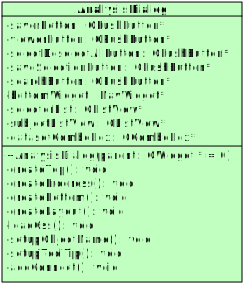
\includegraphics[width=0.6\linewidth] {./Content/Immagini/view/AnalysisDialog.png}
			\caption{Classe AnalysisDialog: attributi e metodi}
			\label{cl_anaDia}
\end{figure}
\paragraph{Descrizione \\}
Classe che rappresenta la finestra di dialogo che viene visualizzata dall'utente durante l'esecuzione dell'analisi.
\paragraph{Utilizzo\\}
La classe viene creata quando l'utente ha scelto il dataset\g{} su cui eseguire l'analisi e le opzioni per la visualizzazione ed esportazione delle Feature\g{}. Mostra all'utente la barra di avanzamento dell'analisi; ad ogni Feature\g{} se precedentemente selezionato, verrà mostrato il risultato ottenuto dall'applicazione della Feature\g{} all'immagine associata al \subject{}. Mette inoltre a disposizione la possibilità di interrompere l'analisi, di proseguire senza più mostrare i risultati delle Feature\g{} oppure di proseguire con l'analisi con le impostazioni scelte.
\paragraph{Classi ereditate\\}
\begin{itemize}
\item Qt::QDialog.
\end{itemize}

\paragraph{\textcolor{black}{Attributi\\}}
%nextButton
\color{teal}\verb!-nextButton: QPushButton*!
\color{black}
\begin{quote}Pulsante che permette di proseguire l'analisi con le impostazioni scelte prima di inziare l'analisi.
\end{quote}
%endButton
\color{teal}\verb! -endButton:QPushButton*!
\color{black} 
\begin{quote}Pulsante che permette di proseguire l'analisi fino alla fine, senza interromperla con la visualizzazione intermedia.
\end{quote}
%progressBar
\color{teal}\verb! -progressBar:QProgressBar*!
\color{black} 
\begin{quote}Identifica la barra di avanzamento che informa l'utente sul tempo mancante alla terminazione dell'analisi.
\end{quote}
%cancelButton
\color{teal}\verb! -cancelButton: QPushButton*!
\color{black}Pulsante che permette l'interruzione dell'analisi in corso.
%%%%%%%%%%%%%%%%%%%% METODI
\paragraph{\textcolor{black}{Metodi\\}}
%costruttore
\color{blue}\verb!- FeatureParams(featureP: QVector<AFeature*>&, parent:QWidget*=0)!
\begin{quote}
\color{black}Costruttore per la classe. \\
\textbf{Argomenti}
\begin{itemize}
\item featureP: QVector<AFeature*>\& \\ Vector di puntatori ad oggetti di tipo \emph{AFeature}. Utilizzato per inizializzare il campo dati \emph{features};
\item parent: QWidget*=0  \\ Puntatore al QWidget padre di FeatureParams.
\end{itemize}
\end{quote}
%LOADCSS
\color{blue}\verb! -loadCss(): void !
\begin{quote}
\color{black} Metodo che ha il compito di caricare il file contentente il css per il widget.
\end{quote} 
%setupObjectName
\color{blue}\verb! -setupObjectName():void!
\begin{quote}
\color{black} Metodo che ha il compito di impostare il nome di ogni oggetto, contenuto nel widget.
\end{quote} 
%setupToolTip
\color{blue}\verb! -setupToolTip():void!
\begin{quote}
\color{black} Metodo che ha il compito di impostare per ogni oggetto i ToolTip necessari per mostrare all'utente, che sta utilizzando \project{}, i suggerimenti e  spiegare a cosa serve quell'oggetto su cui si è posizionato con il cursore.
\end{quote} 
%addConnect
\color{blue}\verb! -addConnect(): void!
\color{black} 
\begin{quote}
Metodo che ha il compito di fissare tutte le istruzioni \emph{connect} degli oggetti che emetteranno un signal\g{} verso il rispettivo controller.
\end{quote} 
%createProgress
\color{blue}\verb! -createProgress(): void !
\begin{quote}
\color{black} Metodo che ha il compito creare il layout contentente la barra di avanzamento dell'analisi.
\end{quote} 
%createTop
\color{blue}\verb! -createTop():void!
\begin{quote}
\color{black} Metodo che ha il compito di creare la parte in alto della finestra di dialogo contenente la visualizzazione dell'anteprima dei risultati intermedi e la barra di avanzamento.
\end{quote} 
%createLayout
\color{blue}\verb! -createLayout():void!
\begin{quote}
\color{black} Metodo che ha il compito di creare il layout per la finestra di dialogo.
\end{quote} 
%createButtom
\color{blue}\verb! -createButtom():void!
\color{black}
\begin{quote}
 Metodo che ha il compito di costruire la parte in basso del widget contenente i pulsanti per l'interazione con l'utente.
\end{quote}
\color{black}
\pagebreak
%%%%%%%%%%%%%%%%%%%
%	HELPVIEW
%%%%%%%%%%%%%%%%%%
\subsubsection{HelpView (class)}
\label{spehelps}
\begin{figure}[!h]
\centering
			\includegraphics[width=0.65\linewidth] {./Content/Immagini/view/HelpView.png}
			\caption{Classe HelpView: attributi e metodi}
			\label{cl_help}
\end{figure}
\paragraph{Descrizione \\}
Classe che rappresenta la guida interattiva che l'utente può consultare durante l'utitilizzo di \project{}. La guida è realizzata in formato HTML (HyperText Markup Language).
\paragraph{Utilizzo\\}
La classe viene creata l'utente preme il pulsante contenuto nelle viste che prevedono l'accesso alla guida interattiva
\paragraph{Classi ereditate\\}
\begin{itemize}
\item Qt::QDialog.
\end{itemize}
\paragraph{\textcolor{black}{Attributi\\}}
%side
\color{teal}\verb! -side:QString!
\color{black} 
\begin{quote}Campo dati che rappresenta il menu laterale per la navigazione tra le sezioni della guida.
\end{quote}
%content
\color{teal}\verb! -content:QString!
\color{black} 
\begin{quote}Campo dati che rappresenta il contenuto della guida interattiva.
\end{quote}
%where
\color{teal}\verb! -where: QString!
\color{black}
\begin{quote}Campo dati che rappresenta la sezione in cui si trova l'utente.
\end{quote}
%%%%%%%%%%%%%%%%%%%% METODI
\paragraph{\textcolor{black}{Metodi\\}}
%costruttore
\color{blue}\verb! +HelpView(parent:QWidget*=0)!
\begin{quote}
\color{black}Costruttore per la classe. \\
\textbf{Argomenti}
\begin{itemize}
\item parent: QWidget*=0  \\ Puntatore al QWidget padre di HelpView.
\end{itemize}
\end{quote}
%createSideBar
\color{blue}\verb! -createSideBar():void!
\begin{quote}
\color{black} Metodo che ha il compito di creare il menu di navigazione a sinistra contenente i topic fulcro della guida in modo da aiutare l'utente alla ricerca efficiente dell'argomento di interesse.
\end{quote} 
%createProgress
\color{blue}\verb! -createContent(): void !
\begin{quote}
\color{black} Metodo che ha il compito creare il layout per il contenuto della guida interattiva.
\end{quote} 
%createTop
\color{blue}\verb! -createTop():void!
\begin{quote}
\color{black} Metodo che ha il compito di creare la parte in alto della finestra di dialogo contenente la vera e propria guida.
\end{quote} 
%setupLayout
\color{blue}\verb! -setupLayout():void!
\begin{quote}
\color{black} Metodo che ha il compito di impostare il layout della finestra di dialogo.
\end{quote} 
%createButtom
\color{blue}\verb! -createButtom():void!
\color{black}
\begin{quote}
 Metodo che ha il compito di costruire la parte in basso del widget contenente i pulsanti per l'interazione con l'utente.
\end{quote}
\color{black}
\pagebreak


